\notechapter{N-20250118}{Schemes Gently: A Guided Tour of Spectrum, Nilpotents, and Local Rings}

\section{A new kind of point}

Classical algebraic geometry studies points satisfying polynomial equations. Scheme theory asks us to enlarge the meaning of point.

For a ring \(R\), define
\[
  \operatorname{Spec}R=\{\mathfrak p\subset R:\mathfrak p\text{ is prime}\}.
\]
This is the spectrum of \(R\). Its points are prime ideals.

At first this feels like a category mistake: ideals are algebraic objects, not points. But this change is exactly what allows geometry to remember generic behavior, arithmetic information, and infinitesimal thickening.

\section{The affine line spectrum}

For \(R=k[x]\), the maximal ideals
\[
  (x-a)
\]
correspond to ordinary points \(a\in k\). But there is also the prime ideal \((0)\), the generic point.

The closure of the generic point is the whole space:
\[
  \overline{\{(0)\}}=\operatorname{Spec}k[x].
\]
This is not Hausdorff behavior, but it is meaningful. The generic point represents the whole irreducible line, while \((x-a)\) represents a closed point.

\begin{center}
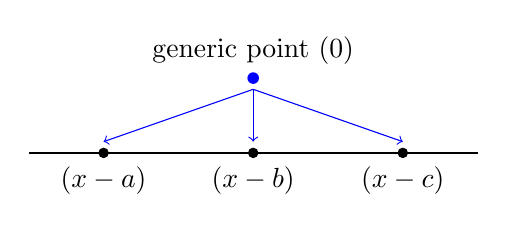
\begin{tikzpicture}[scale=0.95]
  \draw[thick] (-3,0) -- (3,0);
  \foreach \x/\lab in {-2/{(x-a)},0/{(x-b)},2/{(x-c)}} {
    \fill (\x,0) circle (2pt);
    \node[below] at (\x,-.05) {$\lab$};
  }
  \fill[blue] (0,1.0) circle (2.2pt);
  \node[above] at (0,1.05) {generic point $(0)$};
  \draw[->,blue] (0,.85) -- (-2,.15);
  \draw[->,blue] (0,.85) -- (0,.15);
  \draw[->,blue] (0,.85) -- (2,.15);
\end{tikzpicture}
\end{center}

The arrows are suggestive: the generic point specializes to closed points.

\section{Closed sets and distinguished opens}

For an ideal \(I\subset R\), define
\[
  V(I)=\{\mathfrak p\in\operatorname{Spec}R:I\subseteq\mathfrak p\}.
\]
These are closed sets.

For \(f\in R\), define
\[
  D(f)=\{\mathfrak p:f\notin\mathfrak p\}.
\]
This is the region where \(f\) is allowed to be inverted. Distinguished opens are the basic open sets of affine schemes.

\section{Localization is zooming in}

At a prime ideal \(\mathfrak p\), the local ring is
\[
  R_{\mathfrak p}.
\]
It is obtained by inverting every element not in \(\mathfrak p\). The interpretation is simple: near \(\mathfrak p\), functions not vanishing there should be units.

For \(R=k[x]\) and \(\mathfrak p=(x-a)\), the ring
\[
  k[x]_{(x-a)}
\]
contains rational functions whose denominators do not vanish at \(a\). This is the algebraic version of functions defined near \(a\).

\section{The structure sheaf}

A spectrum is not only a topological space. It carries functions. On a distinguished open \(D(f)\), the structure sheaf satisfies
\[
  \mathcal O_{\operatorname{Spec}R}(D(f))=R_f.
\]
The stalk at \(\mathfrak p\) is
\[
  \mathcal O_{\operatorname{Spec}R,\mathfrak p}=R_{\mathfrak p}.
\]
These two formulas are enough to make affine schemes computational rather than mystical.

\section{Nilpotents: invisible but geometric}

Consider
\[
  R=k[x]/(x^2).
\]
The element \(x\) is nonzero but satisfies \(x^2=0\). Topologically, \(\operatorname{Spec}R\) has only one point. Algebraically, it remembers an infinitesimal thickening of that point.

A useful picture is a point with a first-order tangent fuzz. The fuzz cannot be seen as a second classical point, but it can be detected by functions.

This is one of the reasons schemes are powerful: they keep information that ordinary point sets discard.

\section{The arithmetic curve}

The spectrum of the integers has points
\[
  (p)
\]
for prime numbers \(p\), together with the generic point \((0)\). An integer \(n\) vanishes at exactly the primes dividing it:
\[
  V(n)=\{(p):p\mid n\}.
\]
Thus divisibility becomes geometry.

This is one of the most charming features of schemes: number theory begins to resemble geometry, not metaphorically but structurally.


\section{Maximal ideals are not enough}

It is tempting to keep only maximal ideals, because over an algebraically closed field they correspond to ordinary closed points.  But prime ideals contain information about irreducible subspaces.

In \(k[x,y]\), the prime ideal \((x)\) is not a closed point.  It corresponds to the whole \(y\)-axis.  The maximal ideal \((x,y-a)\) is a closed point on that axis.

Thus prime ideals let a scheme contain both points and subvarieties as points of different levels of generality.  This is strange at first, but it is exactly what makes generic points possible.

\section{Specialization as movement from generic to concrete}

In \(\operatorname{Spec}R\), one says that \(\mathfrak q\) specializes to \(\mathfrak p\) when
\[
  \mathfrak q\subseteq\mathfrak p.
\]
The smaller prime is more generic; the larger prime is more special.

For \(k[x]\),
\[
  (0)\subset (x-a),
\]
so the generic point specializes to the closed point \((x-a)\).  This order relation is the topological shadow of ideal containment.

\section{Residue fields}

At a prime \(\mathfrak p\), the local ring \(R_{\mathfrak p}\) has maximal ideal \(\mathfrak pR_{\mathfrak p}\).  The residue field is
\[
  \kappa(\mathfrak p)=R_{\mathfrak p}/\mathfrak pR_{\mathfrak p}.
\]
For a closed point \((x-a)\subset k[x]\), the residue field is \(k\).  For the generic point \((0)\), the residue field is \(k(x)\), the field of rational functions.

This is another way to see the meaning of generic points: at the generic point of the affine line, the coordinate \(x\) is not specialized to a number; it remains a variable.

\section{A tiny nonreduced calculation}

Let
\[
  R=k[\epsilon]/(\epsilon^2).
\]
A function on \(\operatorname{Spec}R\) can have the form
\[
  a+b\epsilon.
\]
The term \(b\epsilon\) is invisible if one only looks at ordinary points, because \(\epsilon\) is nilpotent.  But algebraically it records first-order infinitesimal information.

This is the simplest model of a dual number.  It is also a first hint of why tangent vectors and infinitesimal thickenings are naturally scheme-theoretic.

\section{Reading \texorpdfstring{$\operatorname{Spec}R$}{Spec R} in examples}

The dictionary from this note should be used with actual rings in mind:
\[
\begin{array}{c|c}
\operatorname{Spec}R & \text{prime ideals, including non-maximal ones}\\
D(f) & \text{the part where }f\text{ becomes invertible}\\
R_f & \text{functions allowed to divide by powers of }f\\
R_{\mathfrak p} & \text{functions near the prime }\mathfrak p\\
\kappa(\mathfrak p) & \text{the residue field visible at }\mathfrak p\\
\text{nilpotents} & \text{infinitesimal information not seen by closed points}
\end{array}
\]
For \(\operatorname{Spec}\mathbb Z\), the generic point \((0)\) and the closed points \((p)\) are both needed: localizing at \((p)\) records arithmetic near one prime, while the generic point records information over \(\mathbb Q\).  For \(k[\epsilon]/(\epsilon^2)\), there is only one underlying prime, but the function \(a+b\epsilon\) still contains a first-order term.  These two examples explain why schemes keep more than the set of maximal ideals: they retain specialization, residue fields, and nilpotent thickening.
